En este capítulo se describen los conceptos fundamentales para comprender la metodología propuesta en el capitulo \ref{ch:methodology}. El capítulo es estructurado como sigue. En la sección \ref{sec:mixture_models} se introduce a nivel general los modelos de \textit{clustering} probabilísticos conocidos como \textit{mixture models}. En la sección \ref{sec:topic_models} se describen los modelos de tópicos estáticos LDA y HDP. Finalmente, en la sección \ref{sec:topic_evolution} se explica una metodología que modela la evolución de los tópicos en el tiempo. 

\section{Mixture Models}
\label{sec:mixture_models}

Uno de los supuestos básicos en \textit{clustering} es asumir que cada observación $x_{i}$ pertenece a un solo \textit{cluster} $k$. La asignación a un \textit{cluster} se puede expresar como una variable aleatoria $z_{i}$, donde $z_{i}=k$ significa que $x_{i}$ pertenece al \textit{cluster} $k$. La variable $z_{i}$ no es observada en los datos y se considera una variable oculta. Cada \textit{cluster} posee un parámetro $\phi_{k}$ que codifica su información. La distribución que caracteriza a un solo \textit{cluster} $k$ condicionando en $z_{i}$ es

\begin{align}
    p(x_{i}|z_{i}=k, \phi) = p(x_{i}|\phi_{k})\\
\end{align}

Además, la probabilidad de que una nueva observación pertenezca al \textit{cluster} $k$ se define como 

\begin{align}
    p(z_{i}=k|\pi) = \pi_{k}
\end{align}

Con $\sum_{k}\pi_{k} = 1$, ya que $\pi_{k}$ son probabilidades de eventos mutuamente excluyentes. La distribución de $x_{i}$ es de la forma

\begin{align}
  p(x_{i}) = \sum_{k}p(z_{i}=k|\pi)p(x_{i}|z_{i}=k, \phi) = \sum_{k}\pi_{k}p(x_{i}|\phi_{k})
\end{align}

La distribución $p(x_{i}|\phi_{k})$ se denota $x_{i} \sim F(\phi_{z_{i}})$, donde $F$ es la distribución asociada a las observaciones. \\

Una representación equivalente se obtiene al considerar el parámetro $\phi_{z_{i}}$ usado para generar la observación $x_{i}$ proviene de una distribucion discreta $G$, la cual tiene la forma

\begin{align}
    G(\phi) & = \sum_{k} \pi_{k}\delta_{\phi_{k}}(\phi)
\end{align}

En otras palabras, $G$ es una mezcla de funciones delta, donde la probabilidad de que $\phi$ sea igual a $\phi_{k}$ es $\pi_{k}$. Luego, un \textit{mixture model} se puede  representar como a continuación

\begin{align}
\phi_{z_{i}} & \sim G\\
x_{i} & \sim  F(\phi_{z_{i}})
\end{align}

Un \textbf{Bayesian mixture model} es un \textit{mixture model} con una medida aleatoria para las mezclas. En las secciones \ref{sec:dirichlet}. y \ref{sec:dp} se describen dos \textit{priors} ampliamente usados para construir \textit{bayesian mixture model}: la distribución Dirichlet que permite construir un \textbf{finite mixture model}, donde el número de átomos o \textit{clusters} a descubrir es finito, denotado por $K$ y un \textit{prior} no paramétrico denominado Dirichlet Process (DP), el cual permite construir un \textbf{infinite mixture model}, donde el número de \textit{clusters} no está acotado. 

\subsection{Distribución Dirichlet}
\label{sec:dirichlet}

La distribución Dirichlet \citep{minka2000estimating} es una generalización multivariada de la distribución beta, la cual tiene soporte sobre un \textbf{simplex}, definido por:
\begin{equation}
    S_{K} = \big\{x: 0\leq x_{k} \leq 1, \sum_{k=1}^{K}x_{k}=1\big\}
\end{equation}
Luego, su función de densidad de probabilidad (pdf):

\begin{equation}
    Dir(x|\alpha)=\frac{1}{B(\alpha)}\prod_{k=1}^{K}x_{k}^{\alpha_{k}-1}\mathbb{I}(x\in S_{K})
\end{equation}

, donde $B(\alpha) = B(\alpha_{1}, \ldots, \alpha_{K})$ es la generalización de la función beta a $K$ variables:

\begin{align}
    B(\alpha) \triangleq \frac{\prod_{k=1}^{K}\Gamma(\alpha_{k})}{\Gamma(\alpha_{0})}
\end{align}

, donde $\alpha_{0} \triangleq \sum_{k=1}^{K}\alpha_{k}$.\\

En la Figura \ref{img:dirichlet_distribution} se observa el efecto de los parámetros en la distribución Dirichlet con $K=3$. El parámetro $\alpha_{k}$ controla la \textit{sparsity}, mientras más se acerca a 0 los vectores generados tienen más átomos nulos y se concentra la masa en unas pocas coordenadas, mientras más grande $\alpha_{k}$ la masa más se concentra en el centro (1/3, 1/3, 1/3). Cuando $\alpha_{k}=1$ se tiene una distribución uniforme en el dominio $S_{K}$. Por otro lado, cuando $\alpha$ no es simétrico la masa se concentra proporcionalmente en las coordenadas con $\alpha_{k}$ mayor.\\

\begin{figure}
    \centering
    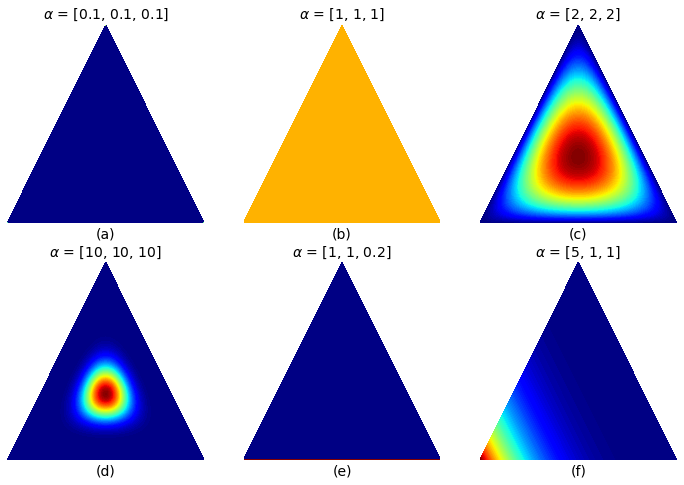
\includegraphics[width=\textwidth]{ch2/dirichlet_simplex.eps}
    \caption{Densidad de la distribución Dirichlet con $K=3$. Define una distribución sobre un \textit{simplex}, el cual puede ser representado por una superficie triangular.}
    \label{img:dirichlet_distribution}
\end{figure}

En general se asume simetría en los parámetros de la distribución Dirichlet de la forma $\alpha_{k}=\frac{\alpha}{K}$, de esta manera $\alpha$ funciona como parámetro de concentración. En la Figura \ref{img:dirichlet_samples} se oberva una realización de una distribución Dirichlet con $\alpha \in \{0.1, 1, 10\}$ y $K\in\{2, 10, 100\}$. En esta figura podemos observar que a mayor $\alpha$ los compenentes del vector $x$ más similares se vuelven, esto es más notorio a mayor dimencionalidad debido a que existen más dimensiones a las que distribuir la masa.\\

La distribución Dirichlet es comúnmente usada en estadística Bayesiana, debido a que es \textit{prior} conjugado de la distribución categórica (multinoulli) y la distribución multinomial. Así, la distribución Dirichlet puede ser utilizado como \textit{prior} en un \textit{finite mixture model} considerando $\pi\sim \text{Dir}(\frac{\alpha}{K}1_{K})$ y $\phi_{k} \sim H$.

\begin{figure}
    \centering
    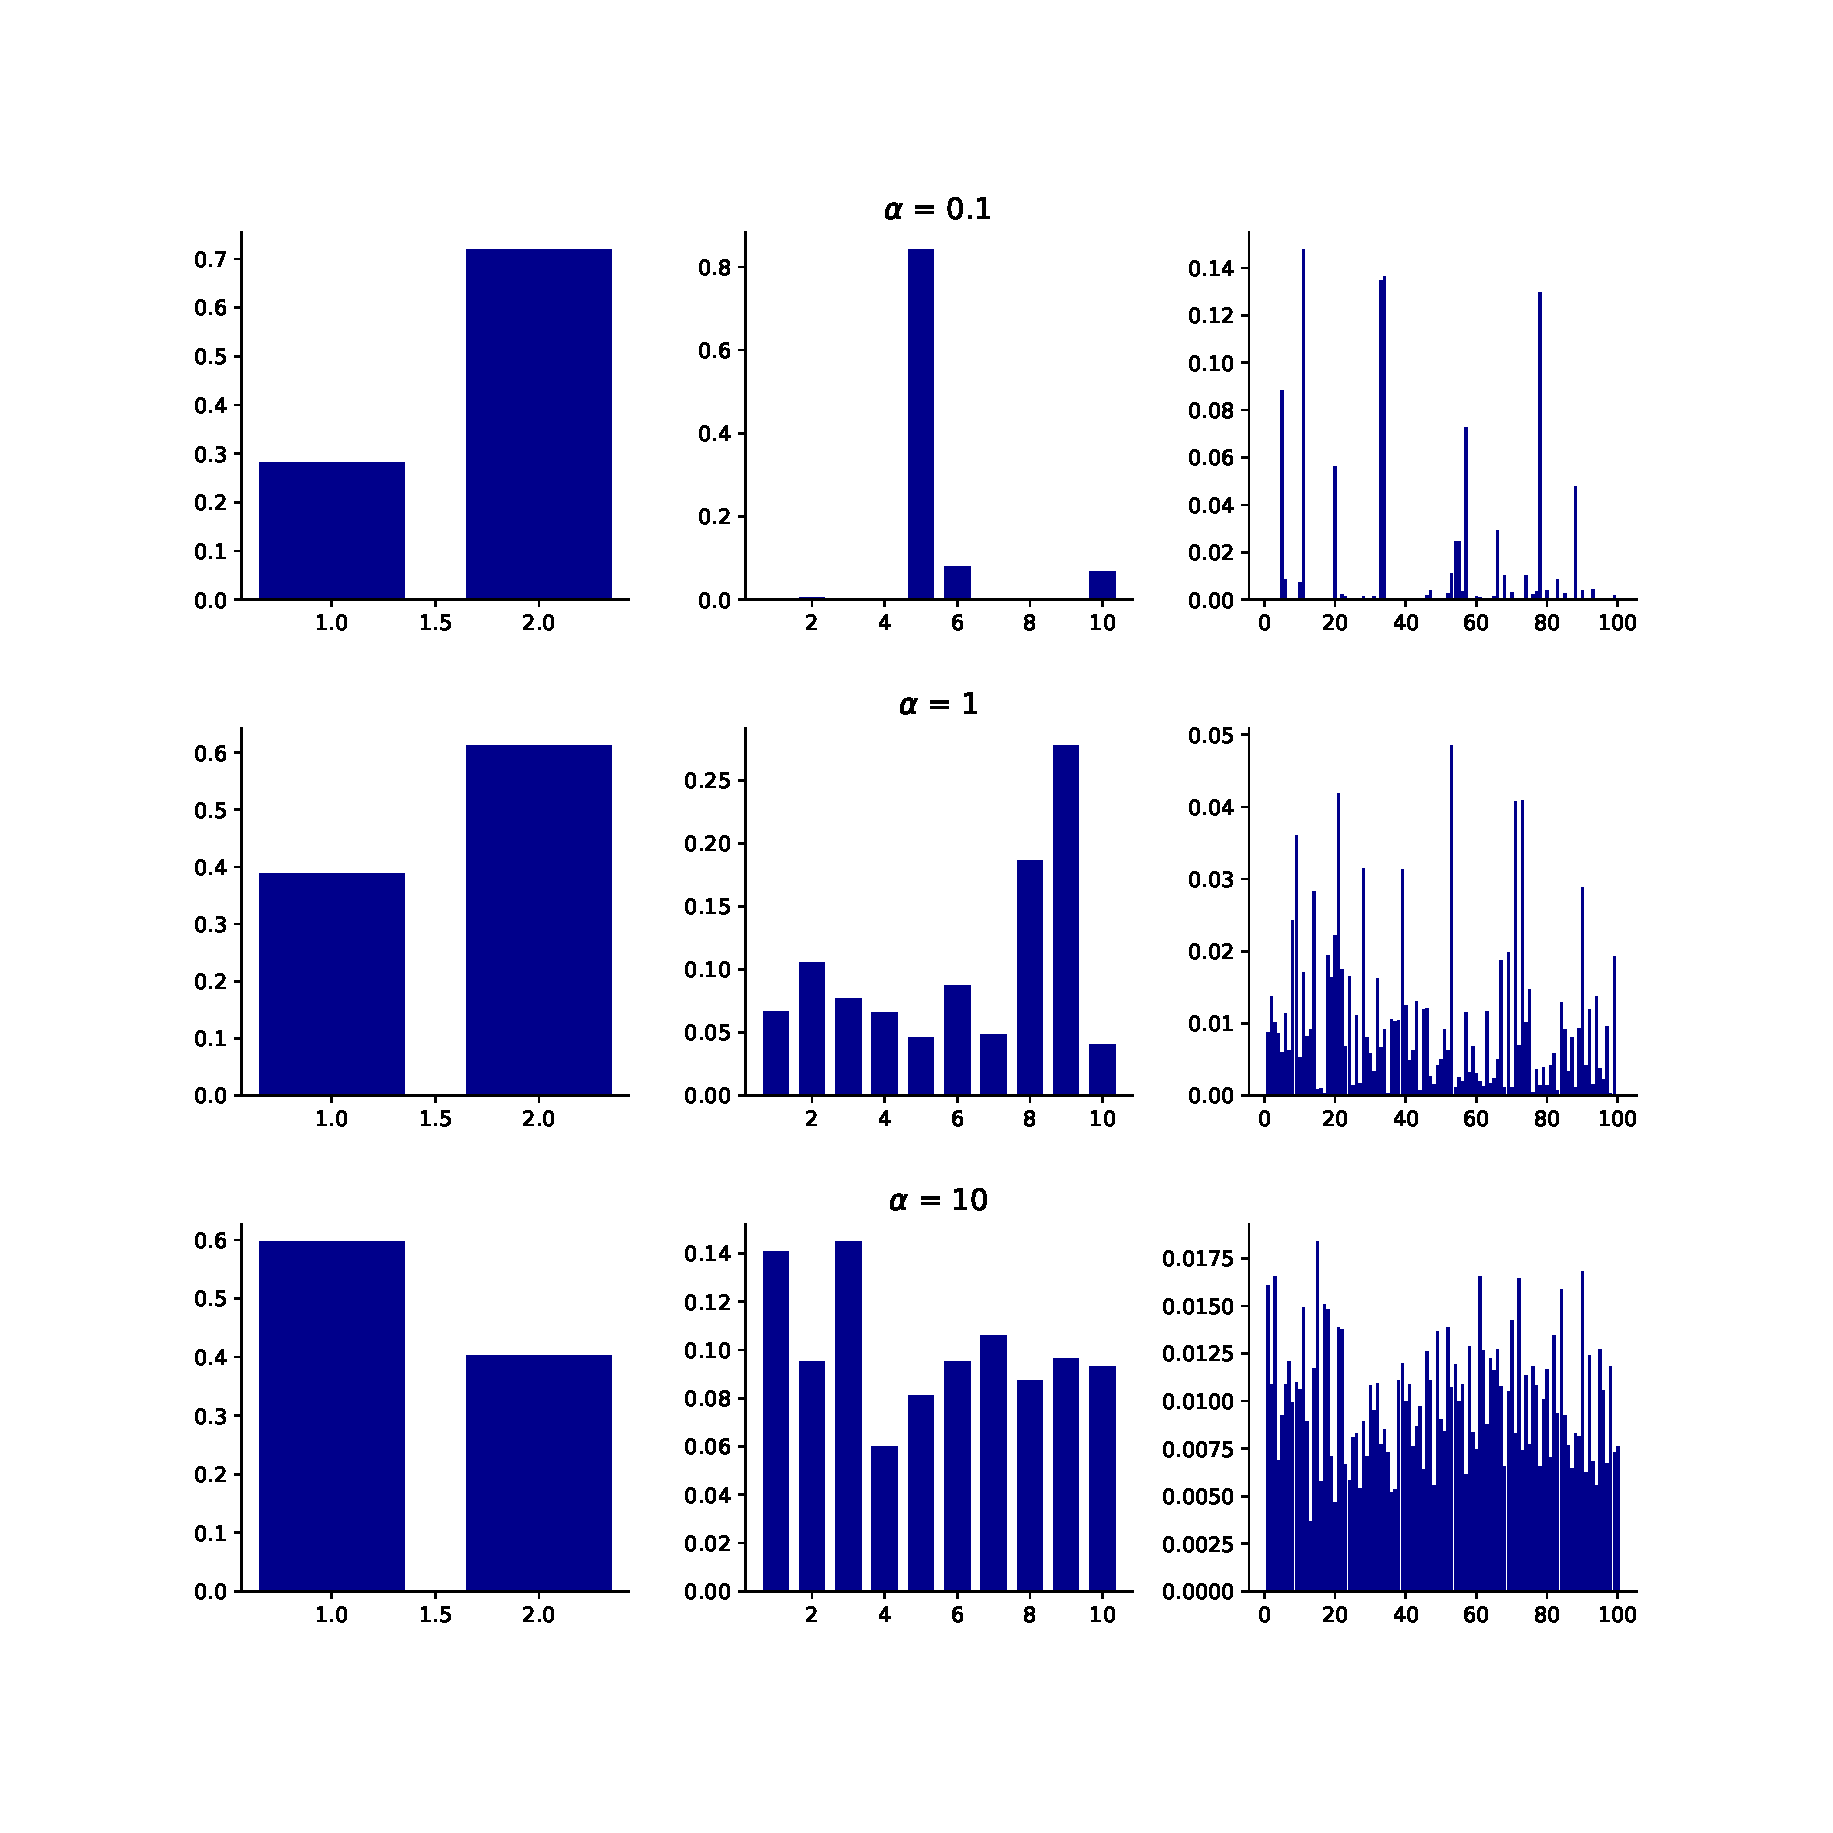
\includegraphics[width=\textwidth]{ch2/dirichlet_samples.eps}
    \caption{Muestra de una distribución Dirichlet simétrica con $\alpha \in \{0.1, 1, 10\}$ y $K\in\{2, 10, 100\}$.}
    \label{img:dirichlet_samples}
\end{figure}

\subsection{Dirichlet Process}
\label{sec:dp}

En un \textit{finite mixture model} se tiene $G(\phi) = \sum_{k=1}^{K} \pi_{k}\delta_{\phi_{k}}(\phi)$, luego al muestrear de $G$, con probabilidad uno se obtendrá exactamente $K$ \textit{clusters}. Sin embargo, es necesario tener un modelo más flexible, que pueda generar un número variable de \textit{clusters}. Una forma de hacer esto es remplazar la distribución discreta $G$ por una medida aleatoria de probabilidad, como el Dirichlet Process \citep{ferguson1973bayesian}, denotado $G\sim \text{DP}(\alpha, H)$.\\

Un \textbf{Dirichlet Process} (DP) es una distribución sobre medidas de probabilidad $G: \Phi \rightarrow \mathbb{R}^{+}$, donde $G(\phi)\geq 0$ y $\int_{\Phi}G(\phi)d\phi=1$. Un DP se define implícitamente por cumplir 

\begin{align}
    G(A_{1}), \ldots, G(A_{K}) \sim \text{Dir}(\alpha H(A_{1}), \ldots, \alpha H(A_{K}))
\end{align}

para cualquier partición finita $(A_{1}, \ldots, A_{k})$ de $\Phi$. En este caso, decimos que $G\sim \text{DP}(\alpha, H)$, donde $\alpha$ es llamado el \textbf{parámetro de concentración} y $H: \Phi \rightarrow \mathbb{R}^{+}$ es llamado la \textbf{medida base}.\\

Como $p(G(A_{1}), \ldots, G(A_{K}))$ es Dirichlet, la distribución marginal en cada partición distribuye beta $\text{Beta}(\alpha H(A_{i}), \alpha \sum_{j\neq i}H(A_{j}))$. El DP es considerado consistentemente definido, ya que si se particiona $\bar{A}_{1}$ en $A_{1}$ y $A_{2}$, entonces $G(\bar{A}_{1})$ y $G(A_{1})+G(A_{2})$ siguen la misma distribución beta. \\

Sea $\pi \sim \text{Dir}(\alpha)$, y $z|\pi  \sim \text{Cat}(\pi)$, si se integra $\pi$ afuera se obtiene la distribución predictiva del modelo Dirichlet-multinoulli:
\begin{align}
    z\sim \text{Cat}(\alpha_{1}/\alpha_{0}, \ldots, \alpha_{K}/\alpha_{0})
\end{align}
donde $\alpha_{0} = \sum_{k}\alpha_{k}$. Es decir, $p(z=k|\alpha)=\alpha_{k}/\alpha_{0}$. Ademas, la posterior de $\pi$ dada una observación viene dada por
\begin{align}
    \pi|z \sim \text{Dir}(\alpha_{1}+\mathbb{I}(z=1), \ldots, \alpha_{K}+\mathbb{I}(z=K))
\end{align}

El DP generaliza el resultado anterior a particiones arbitrarias. Si $G\sim \text{DP}(\alpha, H)$, luego $p(\phi \in A_{i})=H(A_{i})$ y la posterior es

\begin{align}
    p(G(A_{1}), \ldots, G(A_{K})|\phi, \alpha, H) = \text{Dir}(\alpha H(A_{1})+\mathbb{I}(\phi \in A_{1}), \ldots, \alpha H(A_{K})+\mathbb{I}(\phi \in A_{K}))
\end{align}

Esto se mantiene para cualquier conjunto de particiones. Por lo tanto, si observamos multiples muestras $\bar{\phi}_{1:N}\sim G$, la nueva posterior está dada por 

\begin{align}
G|\bar{\phi}_{1:N}, \alpha, H \sim \text{DP}\bigg(\alpha+N, \frac{1}{\alpha+N}\bigg(\alpha H+\sum_{i=1}^{N}\delta_{\bar{\phi}_{i}}\bigg)\bigg)
\end{align}

Por ende el DP define un \textit{prior} conjugado para cualquier espacio medible, donde el parámetro de concentración $\alpha$ es el tamaño de muestro efectivo de la medida base $H$.\\

Existen diferentes perspectivas que ayudan a entender la propiedad de \textit{clustering} de un Dirichlet Process. En la sección \ref{sec:sbp}. y \ref{sec:crp}. se describen dos: el Stick Breaking Process y Chinese Restaurant Process (CRP).

\subsection{Stick Breaking Process}
\label{sec:sbp}

En esta sección se describe una definición constructiva de un DP, conocida como \textit{stick breaking process} \citep{sethuraman1994constructive}. Sea $\pi=\{\pi_{k}\}_{k=1}^{\infty}$ una mezcla de pesos infinita derivada a partir del siguiente proceso:
\begin{align}
    \beta_{k} & \sim \text{Beta}(1, \alpha)\\
    \pi_{k} & = \beta_{k}\prod_{l=1}^{k-1}(1-\beta_{l}) = \beta_{k}(1-\sum_{l=1}^{k-1}\pi_{l})
\end{align}

Esto se suele denotar como $\pi \sim \text{GEM}(\alpha)$, donde GEM representa Griffiths, Engen y McCloskey, ver Figura  \ref{img:stick_breaking} para una ilustración. 

\begin{figure}
    \centering
    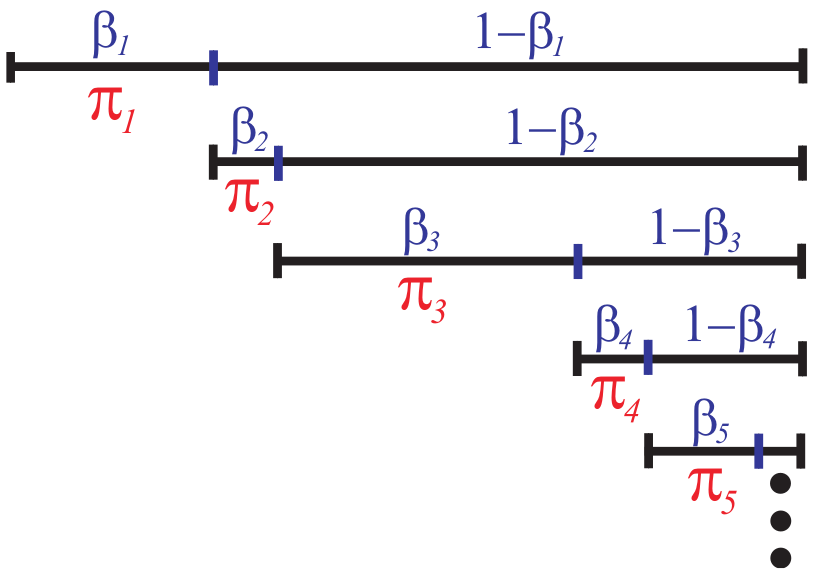
\includegraphics[width=0.6\textwidth]{ch2/stick_breaking.png}
    \caption{Ilustración de \textit{stick breaking process}. Se tiene una barra de largo 1, la cual se rompe en un punto aleatorio $\beta_{1}$, el largo de la pieza restante es llamada $\pi_{1}$, luego recursivamente se rompe la barra restante, así generando $\pi_{2}, \pi_{3}, \ldots$. Fuente: Figura 2.22 de \citep{sudderth2006graphical}.}
    \label{img:stick_breaking}
\end{figure}

Algunos ejemplos de este proceso son mostrados en la Figura \ref{img:dp_samples} (a). A mayor $\alpha$, menos varianza y mayor número de átomos, por el contrario, pequeños valores de $\alpha$ muestran una alta varianza y menor número de átomos. Se puede demostrar que este proceso termina con probabilidad uno, a pesar que el número de elementos que genera incrementa con $\alpha$. Además, el tamaño del componente $\pi_{k}$ decrece en promedio. La distribución $G$ se puede definir como sigue:

\begin{align}
    G(\phi) = \sum_{k=1}^{\infty}\pi_{k}\delta_{\phi_{k}}(\phi)
\end{align}
 
, donde $\pi \sim \text{GEM}(\alpha)$ y $\phi_{k} \sim H$. Es posible demostrar que $G \sim \text{DP}(\alpha, H)$. Como consecuencia de esta construcción, las muestras de un DP son \textbf{discretas con probabilidad uno}. En otras palabras, al muestrear $\bar{\phi_{i}}\sim G$ se observarán valores repetidos, por lo que la mayoría de los datos vendrán de los $\phi_{k}$ con $\pi_{k}$ más largos. En la Figura \ref{img:dp_samples} (b) se muestra un par de medidas aleatorias generadas a partir de un DP con una medida base normal.\\

\begin{figure}
    \centering
    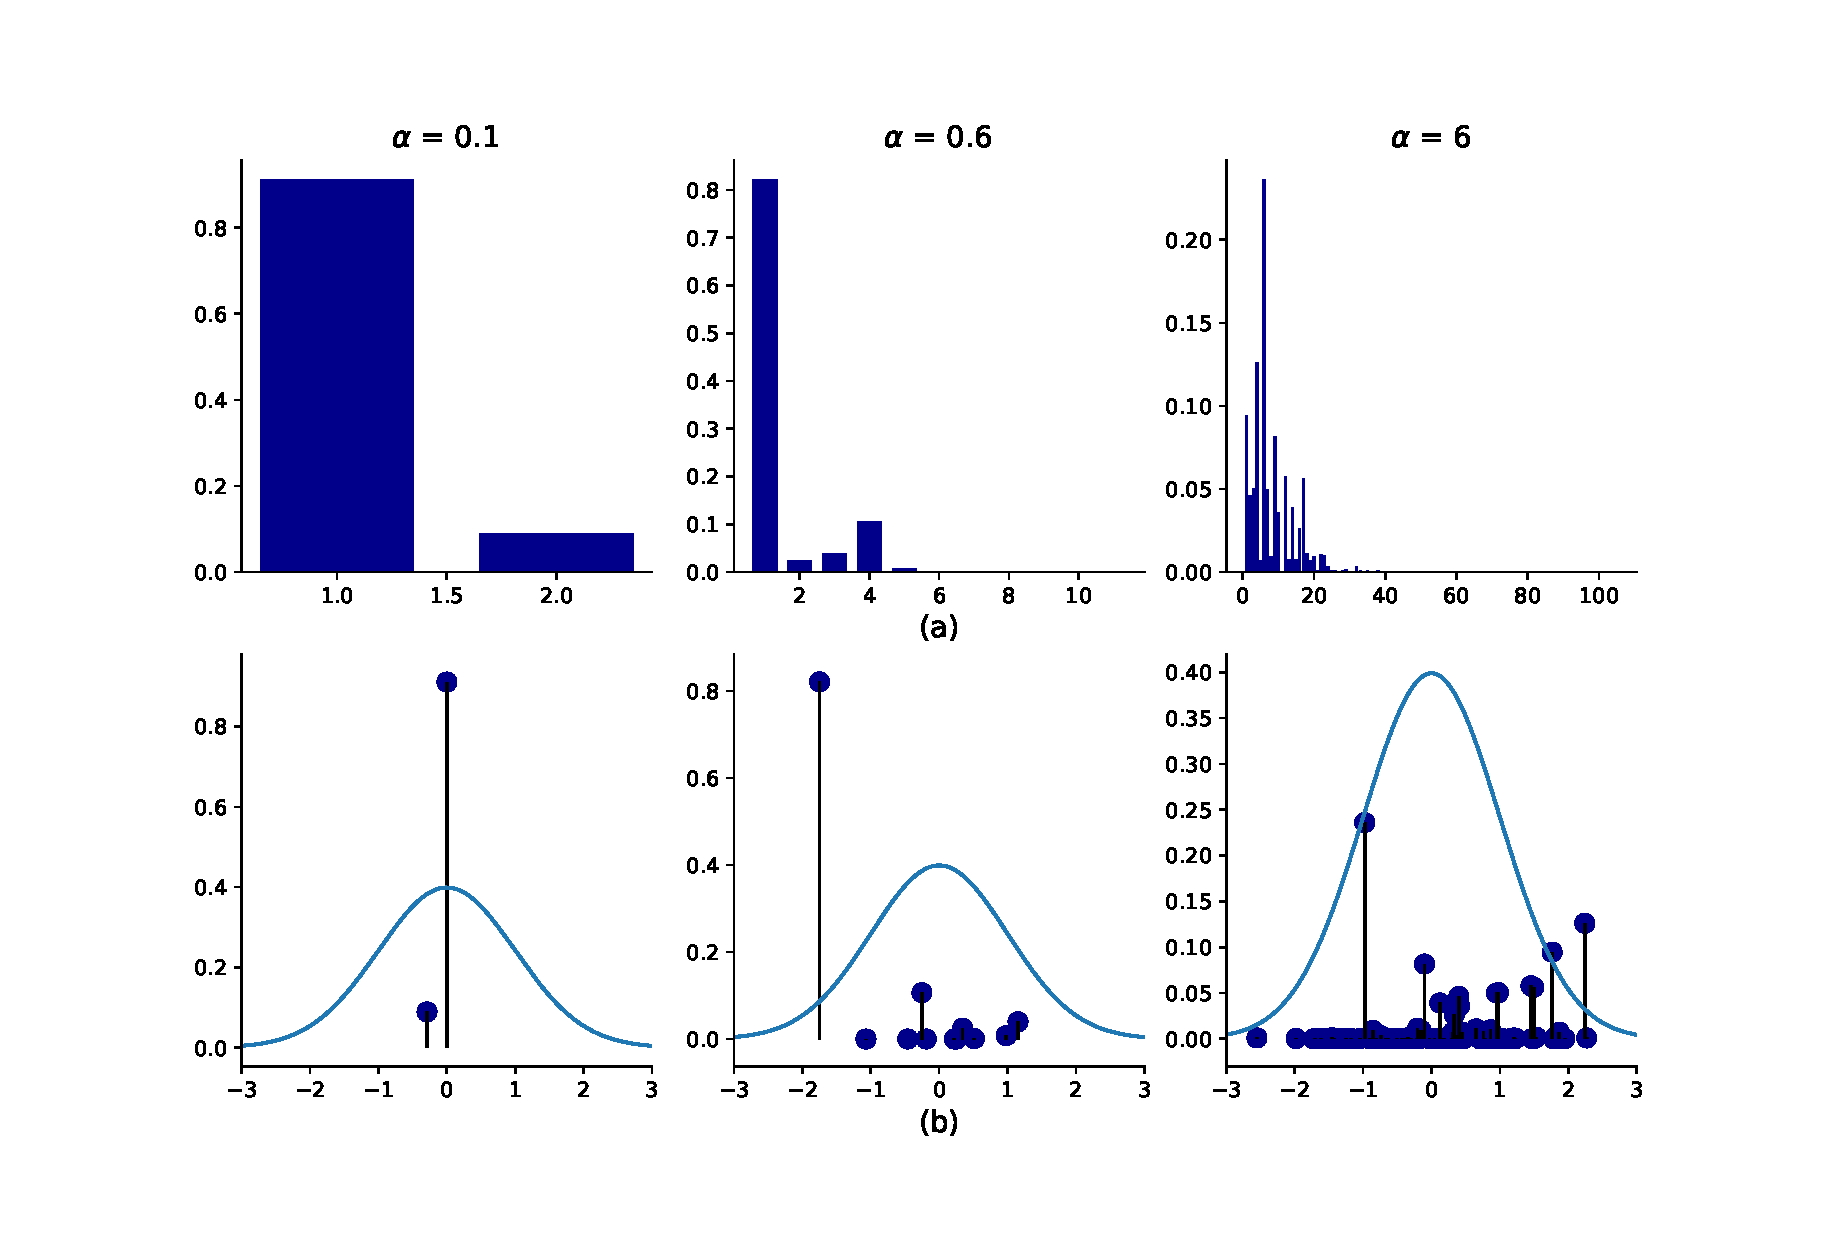
\includegraphics[width=\textwidth]{ch2/dp_samples.eps}
    \caption{(a) Muestras de una distribución GEM con parámetros de concentración $\alpha\in \{0.1, 0.6, 6\}$. (b) Medidas aleatorias generadas a partir de un Dirichlet Process con medida base normal $\mathcal{N}(0,1)$ con parámetros de concentración $\alpha\in \{0.1, 0.6, 6\}$}
    \label{img:dp_samples}
\end{figure}

\subsection{Chinese Restaurant Process}
\label{sec:crp}

Trabajar con infinitos átomos puede ser bastante problemático. Para sortear esta dificultad se puede explotar la propiedad de \textit{clustering} de un DP. Sea $\bar{\phi}_{1:N}\sim G$ observaciones generadas a partir de $G\sim \text{DP}(\alpha, H)$, sea $K$ los distintos valores de $\bar{\phi}_{1:N}$, luego la distribución predictiva condicionada en las $N$ observaciones está dada por

\begin{align}
p(\bar{\phi}_{N+1}=\phi|\bar{\phi}_{1:N}, \alpha, H) = \frac{1}{\alpha+N}\bigg(\alpha H(\phi)+\sum_{k=1}^{K}N_{k}\delta_{\bar{\phi}_{k}}(\phi)\bigg)
\end{align}

donde $N_{k}$ es el número de observaciones previas iguales a $\phi_{k}$. Este esquema de muestreo es llamado \textit{Polya urn} o \textit{Blackwell-MacQueen}. \\

Es más conveniente trabajar con variables discretas $z_{i}$ que especifican cual $\phi_{k}$ usar, así, se define $\bar{\phi}_{i}=\phi_{z_{i}}$. En base a esta expresión se tiene lo siguiente:

\begin{align}
p(z_{N+1}=z|z_{1:N}, \alpha) = \frac{1}{\alpha+N}\bigg(\alpha\mathbb{I}(z=k^{*})+\sum_{k=1}^{K}N_{k}\mathbb{I}(z=k)\bigg)
\end{align}

, donde $k^{*}$ representa un nuevo \textit{cluster} que no ha sido usado aún. Este proceso es denominado Chinese Restaurant Process (CRP) \citep{aldous1985exchangeability}, basado en la oferta aparentemente infinita de mesas en ciertos restaurantes Chinos. La analogía es la siguiente: Las tablas del restaurante son los \textit{clusters}  y los clientes son las observaciones. Cuando una persona entra al restaurante, esta puede escoger sentarse en una tabla existente con probabilidad proporcional al número de personas ya sentadas en esa tabla ($N_{k}$), en otro caso, con una probabilidad decreciente a medida que más personas entran al restaurante (debido a $1/(\alpha +N))$ escogerá sentarse en una nueva tabla $k^{*}$. El resultado de este proceso es una distribución sobre particiones de los naturales, la cual es como una distribución de clientes a tablas.\\

El hecho de que las tablas actualmente ocupadas son más probables de obtener nuevos clientes se suele llamar el fenómeno del \textit{rich get richer}. En efecto, se puede demostrar que la distribución del número de \textit{clusters} que induce este \textit{prior} es básicamente una ley de potencia, donde el número de tablas $K$ con probabilidad 1 se aproxima a $\alpha log(N)$ cuando $N\rightarrow \infty$, mostrando que la complejidad del modelo crece logarítmicamente con el tamaño de los datos.

\section{Modelos de tópicos}
\label{sec:topic_models}
Los modelos de tópicos probabilísticos ayudan a descubrir los temas latentes (\textit{clusters}) en una colección de documentos, como estos temas están conectados unos a otros y cómo cambian en el tiempo. Permiten resumir un gran colección de documentos a través de sus temas y organizarlos entorno a estos.\\

Los modelos probabilísticos tratan un tópico como una distribución de probabilidad discreta sobre el vocabulario del corpus, siendo un práctica habitual interpretar un tópico a partir de sus $N$ palabras más probables. Por ejemplo, con $N=5$ las palabras más probables de un tópico son: \quotes{llaves}, \quotes{domicilio}, \quotes{individuos}, \quotes{casa} y \quotes{porton}, por lo que una etiqueta valida para este tópico podría ser \quotes{portonazo}.\\ 

En \textit{procesamiento del lenguaje natural} (NLP) se suele trabajar bajo la asumpción de \textbf{bag of words} (bolsa de palabras), es decir, tanto los documentos como las palabras son tratadas como intercambiables. Es importante hacer notar que itercambiabilidad no es equivalente a que las variables aleatorias son independientes e identicamente distribuidas. Más bien, intercambiabilidad esencialmente puede ser interpretado como condicionalmente independientes e identicamente distribuidas, donde el condicionamiento es con respecto a los parámetros de una distribución de probabilidad. Por lo tanto, el supuesto de intercambiabilidad es claramente un supuesto de simplificación cuya principal justificación es la construcción de algoritmos computacionales más eficientes.\\

Un \textit{mixture model} que trabaja bajo la asumpción de \textit{bag of words} es \textit{mixture of unigrams} \citep{nigam2000text}, el cual asume que todos los documentos provienen de un solo \textit{cluster} dentro de un conjunto finito de $K$ \textit{clusters}. Los documentos de un \textit{cluster} discuten solo un tópico particular $z$, y cada tópico $z$ está asociado a una distribución categórica. Así, la verosimilitud de observar un documento $d$ es

\begin{align}
    w|z &\sim \text{Cat}(\theta_{z})\\
    p(w_{1}, \ldots, w_{N_{d}}) &= \sum_{z=1}^{K}p(z)\prod_{i=1}^{N_{d}}p(w_{i}|z)
\end{align}

En las secciones \ref{sec:lda}-\ref{sec:hdp} se describe en detalle dos modelos de tópicos probabilísticos, Latent Dirichlet Allocation (LDA) y Hierarchical Dirichlet Process (HDP), considerado la generalización no parámetrica de LDA, donde el número de tópicos a descubrir no está acotado y se infiere a partir del corpus.\\

En comparación a \textit{mixture of unigrams}, LDA y HDP suponen que las palabras de un documento provienen de un mismo \textit{mixture model}, donde a nivel corpus los \textit{mixture models} comparten parámetros, que vienen siendo los tópicos, pero las \textit{mixtures of topics} son específicas de cada documento. Esto permite relajar la asumpción de que cada documento es generado por un solo tópico, debido a que cada palabra proviene de algún tópico, por lo que un documento puede tener presencia de más de un tema.\\

\subsection{Latent Dirichlet Allocation}
\label{sec:lda}

En Latent Dirichlet Allocation (LDA) \citep{blei2003latent} cada tópico es una distribución de probabilidad sobre un vocabulario fijo $V$. Cada documento $d$ tiene su propia mezcla de tópicos $\pi_{d}$. La asignación $z_{d,n}\in\{1, \ldots, K\}$  de de una palabra $n$ a un tópico $z$ es dibujada a partir de $\pi_{d}$. El modelo completo es como sigue

\begin{align}
    \phi_{k}|\eta \quad & \sim\quad \text{Dir}(\frac{\eta}{|V|}1_{|V|})\\
    \pi_{d}|\alpha \quad & \sim \quad \text{Dir}(\frac{\alpha}{K}1_{K})\\
    z_{d,n}|\pi_{d} \quad & \sim \quad \text{Cat}(\pi_{d})\\
    w_{d,n}|z_{d,n}, \phi_{1:K} \quad & \sim \quad \text{Cat}(\phi_{z_{d,n}})
\end{align}

Esto es ilustrado en la Figura \ref{img:lda}.
\begin{figure}
  \centering
  \tikz{ %

    \node[latent, dashed] (alpha) {$\alpha$} ; %
    \node[latent, right=of alpha] (pi) {$\pi_{d}$} ; %
    \node[latent, right=of pi] (z) {$z_{d,n}$} ; %
    \node[obs, right=of z] (w) {$w_{d,n}$}   ; %
    \node[latent, right=of w] (phi) {$\phi_{k}$} ; %
    \node[latent, right=of phi, dashed] (eta) {$\eta$} ;%
    \plate[inner sep=0.25cm, xshift=-0.12cm, yshift=0.12cm] {plate1} {(z) (w)} {$N_{d}$}; %
    \plate[inner sep=0.25cm, xshift=-0.12cm, yshift=0.12cm] {plate2} {(pi) (plate1)} {$D$}; %
    \plate[inner sep=0.25cm, xshift=-0.12cm, yshift=0.12cm] {plate3} {(phi)} {$K$}; %
    \edge {alpha} {pi} ; %
    \edge {pi} {z} ; %
    \edge {z,phi} {w} ; %
    \edge {eta} {phi} ; %
  }
\caption{Representación gráfica de LDA: círculos denotan variables aleatorias, círculos abiertos denotan parámetros, círculos sombreados denotan variables observadas y los platos indican replicación.}
\label{img:lda}
\end{figure}

La probabilidad conjunta del modelo:
\begin{equation}
    p(\phi, \pi, z, w|\alpha, \eta)= \prod_{k=1}^{K}p(\phi_{k}|\eta)\prod_{d=1}^{D}p(\pi_{d}|\alpha)\prod_{n=1}^{N_{d}}p(z_{d,n}|\pi_{d})p(w_{d,n}|\phi_{1:K}, z_{d,n})
\end{equation}

La distribución a posterior:
\begin{equation}
    p(\phi, \pi, z|w, \alpha, \eta) = \frac{p(\phi, \pi, z, w|\alpha, \eta)}{p(w|\alpha, \eta)}
\end{equation}

La distribución posterior es computacionalmente intratable para inferencia exacta, debido a que para normalizar la distribución se debe marginalizar sobre todas las variables ocultas y escribir la constante de normalización en términos de los parámetros del modelo. Para poder computar la posterior es necesario utilizar algoritmos de inferencia aproximada, donde el enfoque habitual es Markov Chain Monte Carlo (MCMC) \citep{andrieu2003introduction} e Inferencia Variacional (VI) \citep{blei2017variational}. En \citep{blei2003latent} se propone un algoritmo basado en VI y en \citep{griffiths2004finding} en MCMC.\\

Una representación equivalente en LDA sería generar cada palabra de un documento $d$ a partir de un tópico dibujado por una distribución $G_{d}$,

\begin{align}
    \phi_{k}|\eta \quad & \sim \quad \text{Dir}(\frac{\eta}{|V|}1_{|V|})\\
    \pi_{d}|\alpha \quad & \sim \quad \text{Dir}(\frac{\alpha}{K}1_{K})\\
    G_{d}(\phi)\quad & = \quad \sum_{k=1}^{K}\pi_{d, k}\delta_{\phi_{k}}(\phi)\\
    \phi_{d,n}|\pi_{d}, \phi_{1:K} \quad & \sim \quad G_{d}\\
    w_{d,n}|\phi_{d,n} \quad & \sim \quad  \text{Cat}(\phi_{d,n})
\end{align}

\subsection{Hierarchical Dirichlet Process}
\label{sec:hdp}

Hierarchical Dirichlet Process (HDP)\citep{teh2005sharing} es un \textit{prior} jerárquico no paramétrico, el cual está formado por un DP cuya medida base $G_{0}$ es dibujada a partir de un DP. En el caso de modelamiento de tópicos, se tiene un medida global $G_{0}$ a nivel corpus que es dibujada a partir de un DP con medida base Dirichlet y una medida $G_{d}$ para cada documento que es dibujada a partir de un DP con medida base $G_{0}$. El modelo completo es como sigue

\begin{align}
   H \quad &= \quad \text{Dir}(\frac{\eta}{|V|}1_{|V|})\\
   G_{0}|\gamma, H \quad &\sim \quad \text{DP}(\gamma, H)\\
   G_{d}|\alpha_{0}, G_{0} \quad &\sim \quad \text{DP}(\alpha_{0}, G_{0})\\
   \phi_{d,n}|G_{d} \quad &\sim \quad G_{d}\\
   w_{d,n}|\phi_{d,n} \quad &\sim \quad \text{Cat}(\phi_{d,n})
\end{align}

Esto es ilustrado en la Figura \ref{img:hdp}.

\begin{figure}
  \centering
  \tikz{ %
    \node[latent, dashed] (H) {$H$} ; %
    \node[latent, right=of H] (G0) {$G_{0}$} ; %
    \node[latent, above= of G0, dashed] (gamma) {$\gamma$} ; %
    \node[latent, right=of G0] (Gd) {$G_{d}$} ; %
    \node[latent, above= of Gd, dashed] (alpha0) {$\alpha_{0}$} ; %
    \node[latent, right= of Gd] (phi) {$\phi_{d,n}$} ; %
    \node[obs, right=of phi] (w) {$w_{d,n}$}   ; %
    \plate[inner sep=0.25cm, xshift=-0.12cm, yshift=0.12cm] {plate1} {(phi) (w)} {$N_{d}$}; %
    \plate[inner sep=0.25cm, xshift=-0.12cm, yshift=0.12cm] {plate2} {(Gd) (plate1)} {$D$}; %
    \edge {H, gamma} {G0} ; %
    \edge {G0, alpha0} {Gd} ; %
    \edge {Gd} {phi} ; %
    \edge {phi} {w} ; %
  }
\caption{Representación gráfica de HDP: círculos denotan variables aleatorias, círculos abiertos denotan parámetros, círculos sombreados denotan variables observadas y los platos indican replicación.}
\label{img:hdp}
\end{figure}

La discretitud a nivel corpus de $G_{0}$ asegura que todos los documentos comparten el mismo conjunto de tópicos (\textit{mixture components}). A nivel documento $G_{d}$ hereda los tópicos de $G_{0}$, pero los pesos de cada tópico (\textit{mixture proportions}) es específica del documento.\\


\subsubsection{Stick Breaking Construction}
Aplicando \textit{stick breaking construction} se tiene que para el DP dibujado a nivel corpus la siguiente representación:

\begin{align}
    \beta_{k}^{'} \quad &\sim \quad \text{Beta}(1, \gamma) \\
    \beta_{k} \quad &= \quad \beta_{k}^{'}\prod_{l=1}^{k-1}(1-\beta_{l}^{'})\\
    \phi_{k} \quad &\sim \quad H  \\
    G_{0}(\phi) \quad &= \quad \sum_{k=1}^{\infty}\beta_{k}\delta_{\phi_{k}}(\phi)
\end{align}

Así, $G_{0}$ es discreto y tiene soporte en los átomos $\phi = \{\phi\}_{k=1}^{\infty}$ con pesos $\beta=\{\beta_{k}\}_{k=1}^{\infty}$, siendo la distribución de $\beta$ escrita como $\beta \sim \text{GEM}(\gamma)$. La construcción a nivel documento de $G_{d}$ es:

\begin{align}
    \pi_{d,k}^{'} \quad &\sim \quad \text{Beta}\big(\alpha_{0}\beta_{k}, \alpha_{0}\big(1-\sum_{l=1}^{k}\beta_{l}\big)\big)\\
    \pi_{d,k} \quad &= \quad \pi_{d,k}^{'}\prod_{l=1}^{k-1}(1-\pi_{d,l}^{'})\\
    G_{d}(\phi) \quad &= \quad\sum_{k=1}^{\infty}\pi_{d,k}\delta_{\phi_{k}}(\phi)\\
    \phi_{d,n}|\pi_{d}, \phi_{1:\infty} \quad &\sim \quad G_{d}
\end{align}

Donde $\phi = \{\phi_{k}\}_{k=1}^{\infty}$ son los mismos átomos de $G_{0}$. Esto es ilustrado en la Figura \ref{img:hdp_sbc}.

%stick breaking
\begin{figure}
  \centering
  \tikz{ %
    \node[latent] (beta) {$\beta$} ; %
    \node[latent, above= of beta, dashed] (gamma) {$\gamma$} ; %
    \node[latent, right=of beta] (pi) {$\pi_{d}$} ; %
    \node[latent, above= of pi, dashed] (alpha0) {$\alpha_{0}$} ; %
    \node[latent, right= of pi] (z) {$z_{d,n}$} ; %
    \node[obs, right=of z] (w) {$w_{d,n}$}   ; %
    \node[latent, right=of w] (phi) {$\phi$} ; %
    \node[latent, above=of phi, dashed] (H) {$H$} ; %
    \plate[inner sep=0.25cm, xshift=-0.12cm, yshift=0.12cm] {plate1} {(z) (w)} {$N_{d}$}; %
    \plate[inner sep=0.25cm, xshift=-0.12cm, yshift=0.12cm] {plate2} {(pi) (plate1)} {$D$}; %
    \plate[inner sep=0.25cm, xshift=-0.12cm, yshift=0.12cm] {plate3} {(phi)} {$K (\infty)$}; %
    \edge {gamma} {beta} ; %
    \edge {beta, alpha0} {pi} ; %
    \edge {pi} {z} ; %
    \edge {z, phi} {w} ; %
    \edge {H} {phi} ; %
  }
\caption{Representación gráfica de la construcción stick-breaking de HDP: círculos denotan variables aleatorias, círculos abiertos denotan parámetros, círculos sombreados denotan variables observadas y los platos indican replicación.}
\label{img:hdp_sbc}
\end{figure}

\subsubsection{Chinese Restaurant Franchise Process}

Una construcción alternativa de HDP es conocida bajo el nombre de \textit{Chinese Restaurant Franchise Process} (CRF), una extensión del CRP, que permite compartir un conjunto de platos a través de una cadena de restaurantes Chinos. La analogía es la siguiente, se tienen $D$ restaurantes, cada uno con $N_{d}$ clientes que se sientan en tablas $t_{d,i}$, en cada tabla es servido un único plato $\phi_{k}\sim H$ a partir de un menú común para todos los restaurantes. \\

Sea $m_{dk}$ el número de tablas sirviendo el plato $k$ en el restaurante $d$, así $m_{d.}$ representa el número de tablas en el restaurante $d$, $m_{.k}$ representa el número de tablas sirviendo el plato $k$, y $m_{..}$ el número total de tablas ocupadas. Al integrar $G_{d}$ la probabilidad condicional del cliente $i$-ésimo este en la tabla $t$ se puede escribir como sigue:

\begin{align}
p(t_{di}=t|t_{d1}, \ldots, t_{d,i-1}, \alpha_{0}, G_{0}) = \frac{1}{\alpha_{0}+i-1}\bigg(\alpha_{0}\mathbb{I}(t=t^{*})+\sum_{t^{'}=1}^{m_{d.}}N_{dt^{'}}\mathbb{I}(t=t^{'})\bigg)
\end{align}

donde $N_{dt^{'}}$ representa los clientes del restaurante $d$ que están sentados en la tabla $t^{'}$. Con probabilidad proporcional a los clientes sentados en la tabla $t$ los clientes del restaurante se sentarán en esta y con probabilidad proporcional a $\alpha_{0}$ en una nueva. Una vez todos los clientes estan sentados se tiene una partición sobre $\phi_{d1}, \ldots, \phi_{dN_{d}}$ para cada documento $d$. Luego, al integrar afuera $G_{0}$ se obtiene:

\begin{align}
    p(z_{dt}=z|z_{11}, z_{12}, \ldots, z_{d1}, \ldots, z_{d, t-1}|\gamma, H) = \frac{1}{\gamma+m_{..}}\bigg(\gamma\mathbb{I}(z=k^{*})+\sum_{k=1}^{K}m_{.k}\mathbb{I}(z=k)\bigg)
\end{align}

en este caso se tiene que la tabla $t$ del restaurante $d$ con probabilidad proporcional al número de tablas que sirven el plato $k$ ($m_{.k}$) servirá el plato $k$ y con probabilidad proporcional a $\gamma$ servirá un nuevo plato.\\

Por último, al igual que LDA la distribución posterior de HDP es intratable, por lo que se debe recurrir a técnicas de inferencia aproximada. En \citep{teh2005sharing} se propone un algoritmo basado en MCMC bajo la construcción CRF de un HDP. 

\section{Modelamiento de la evolución de los tópicos en el tiempo}
\label{sec:topic_evolution} 

En \citep{wilson2011tracking} y \citep{beykikhoshk2018discovering} se propone una metodología que permite capturar los dinámismos mencionados usando LDA y HDP respectivamente. Donde se propone dividir el corpus en $T$ épocas, en cada época se entrena un modelo de tópicos estático, obteniéndose así $T$ conjuntos de tópicos $\phi=\{\phi_{1}, \ldots, \phi_{T}\}$, con $\phi_{t}=\{\phi_{t,1}, \ldots, \phi_{t,K_{t}}\}$ el conjunto de tópicos que describen la época $t$, y $K_{t}$ el número de tópicos inferido en esa época. Una vez descubiertos los tópicos se hace uso de medidas de distancia o similitud para relacionar tópicos de épocas adyacentes.\\

En las secciones \ref{sec:similarity_graph}-\ref{sec:automatic_construction} se describe la metodología propuesta en \citep{beykikhoshk2018discovering} para relacionar los tópicos descubiertos de épocas adyacentes.

\subsection{Gráfo de similitud temporal}
\label{sec:similarity_graph}
Para relacionar los tópicos de una época es necesario contar una medida de similitud $\rho \in [0,1]$, con esta médida de similitud se puede construir un gráfo, donde los nodos son los tópicos de una época y los arcos relacionan tópicos de una época con la siguiente, siendo el peso del arco la similitud entre los tópicos. Una vez construido el grafo se eliminan las conexiones débiles en base a un umbral $\zeta \in [0,1]$ a definir, reteniendo solo aquellas conexiones entre tópicos suficientemente similares entre épocas adyacentes, matemáticamente se poda el arco entre los tópicos $\phi_{t,i}$ y $\phi_{t+1,j}$ si $\rho(\phi_{t,i}, \phi_{t+1,j})\leq \tau.\\

Está metodología permite detectar desaparición de un tópico, nacimiento de un nuevo tópico, como también división o fusión entre diferentes tópicos. A continuación se define en detalle cada uno de estos dinamismos:

\begin{itemize}
    \item \textbf{Nacimiento de un tópico:} Si un tópico no tiene ningún arco entrante, por ejemplo, en la Figura \ref{img:graph} el tópico $\phi_{j+2}$ en $t$.
    \item \textbf{Muerte de un tópico:} Si un tópico no tiene ningún arco saliente, por ejemplo, en la Figura \ref{img:graph} el tópico $\phi_{j}$ en $t$.
    \item \textbf{Evolución de un tópico:} Cuando un tópico tiene exactamente un arco de entrada y salida, por ejemplo, en la Figura \ref{img:graph} entre las épocas $t$ y $t+1$ se tiene que el tópico $\phi_{j+2}$ evoluciona del tópico $\phi_{k+1}$.
    \item \textbf{División de un tópico:} Si un tópico tiene más de un arco saliente, por ejemplo, en la Figura \ref{img:graph} el tópico $\phi_{i}$ de $t-1$ se divide en $t+1$ en los tópicos $\phi_{j}$ y $\phi_{j+1}$.
    \item \textbf{Fusión de un tópico:} Cuando un tópico tiene más de un arco entrante, este tipo de tópicos también pueden ser entendidos como un nuevo tópico, por ejemplo, en la Figura \ref{img:graph} los tópicos $\phi_{i}$ y $\phi_{i+1}$ de $t-1$ forman al tópico $\phi_{j+1}$ en $t$.
\end{itemize}

\begin{figure}
    \centering
    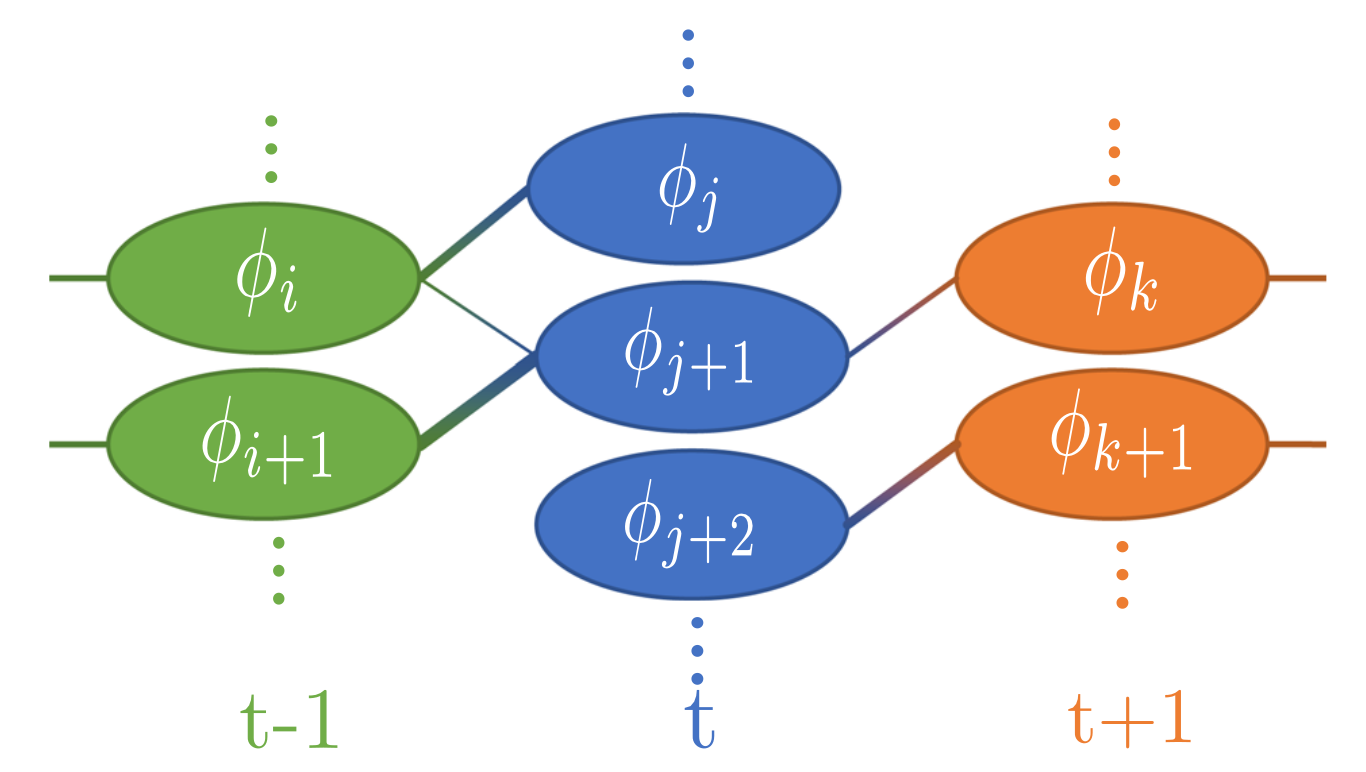
\includegraphics[width=0.8\textwidth]{ch2/similarity_graph.png}
    \caption{Ilustración conceptual del grafo de similitud que modela la dinámica de los tópicos en el tiempo. Un nodo corresponde a un tópico en una época específica; el ancho de los arcos es proporcional a la similitud entre los tópicos, arcos ausentes fueron eliminados por presentar una similitud menor a un umbral. Fuente:  Figura 3 de \citep{beykikhoshk2018discovering}}
    \label{img:graph}
\end{figure}

\subsection{Construcción automática del grafo de similitud}
\label{sec:automatic_construction}

Un aspecto relevante de esta metodología es definir el úmbral de corte, el cual no es fácilmente interpretable, además el úmbral depende de la médida de similitud escogida, dificultando así la comparación entre médidas de similitud. En \citep{beykikhoshk2018discovering} proponen una alternativa más interpretable para definir el úmbral, para esto estiman la función de densidad acumulada (cdf) del grafo inicial, donde todos los nodos de una época están conectados con todos los nodos de la época adyacente, al que de ahora en adelante se denota grafo \textit{fully-connected}. \\

Sea $F_{p}$ la cdf sobre las similitudes del grafo inicial, luego sea $\zeta \in [0,1]$ el punto operante de la cdf, luego se elimina el arco entre los tópicos $\phi_{t,i}$ y $\phi_{t+1,j}$ si $\rho(\phi_{t,i}, \phi_{t+1,j})\leq F_{p}^{-1}(\zeta)$, donde  $F_{p}^{-1}(\zeta)$ es el cuantil $\zeta$ de $F_{p}$. En \ref{img:cdf_sim} se tiene una ilustración para tres médidas de similitud, en esta se observa que la elección arbitraria del úmbral de corte depende fuertemente de la médida de similitud escógida, por lo que la elección en base a la cdf puede ser más apropiada.

\begin{figure}
    \centering
    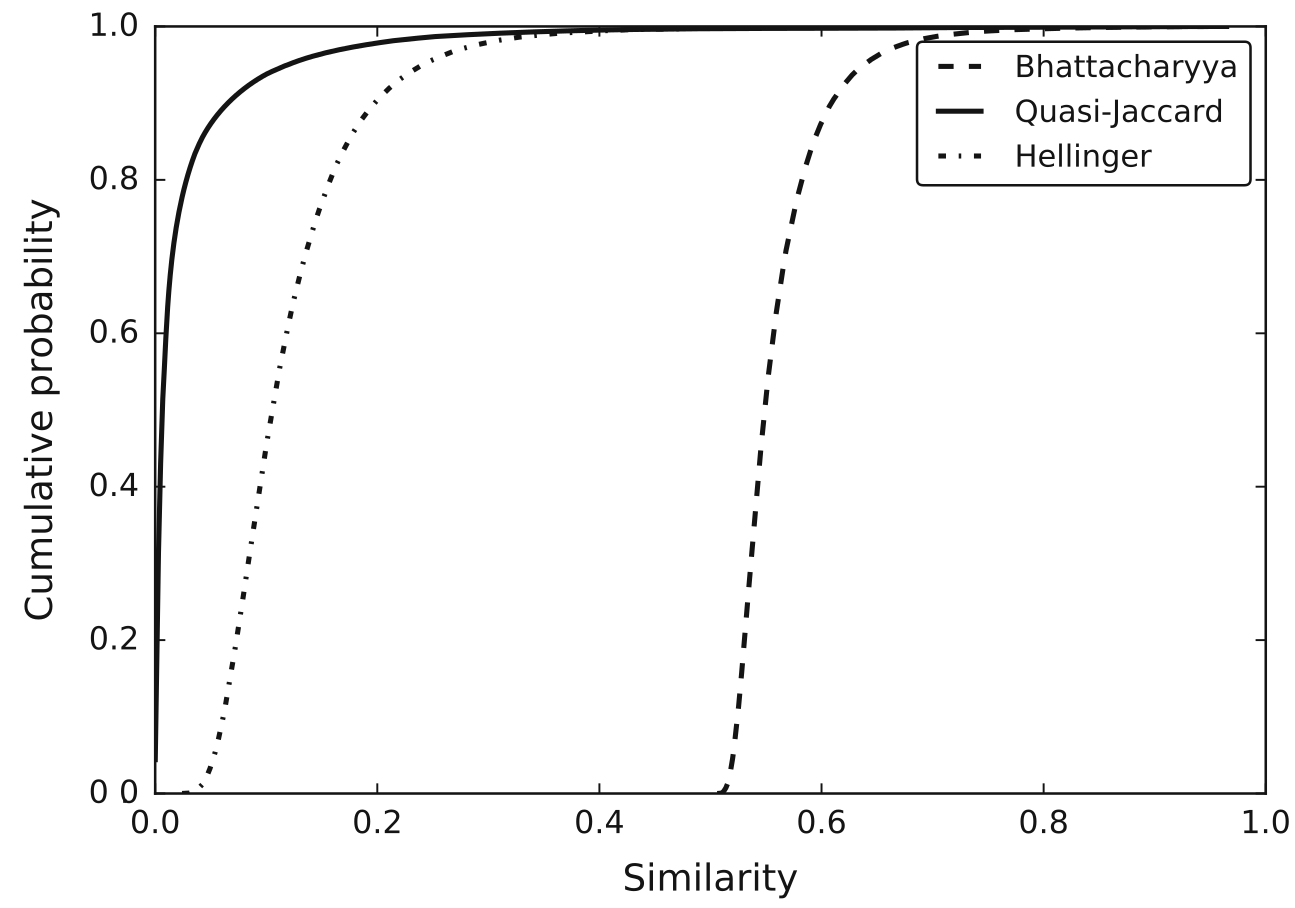
\includegraphics[width=0.8\textwidth]{ch2/cdf_sim.png}
    \caption{Estimación empírica de la función de densidad acumulada (cdf) de la similitud entre tópicos de épocas adyacentes en un grafo \textit{fully-connected} para tres medidas de similitud. Fuente: Figura 4 \citep{beykikhoshk2018discovering}.}
    \label{img:cdf_sim}
\end{figure}
